\documentclass[dvips, lscape]{foils}
%\documentclass[dvips, french]{slides}
\textwidth 18cm
\textheight 25cm 
\topmargin -1cm 
\oddsidemargin  -1cm 
\evensidemargin  -1cm

% Maths
\usepackage{amsfonts, amsmath, amssymb}
% \newcommand{\Acal}{\mathcal{A}}
% \newcommand{\Ccal}{\mathcal{C}}
\newcommand{\Dcal}{\mathcal{D}}
\newcommand{\Ecal}{\mathcal{E}}
\newcommand{\Ncal}{\mathcal{N}}
\newcommand{\Pcal}{\mathcal{P}}
% \newcommand{\Ucal}{\mathcal{U}}
\newcommand{\Hbf}{{\bf H}}
\newcommand{\Bcal}{\mathcal{B}}
\newcommand{\Lcal}{\mathcal{L}}
\newcommand{\Tcal}{\mathcal{T}}
\newcommand{\Ucal}{\mathcal{U}}
\newcommand{\alphabf}{\mbox{\mathversion{bold}{$\alpha$}}}
\newcommand{\betabf}{\mbox{\mathversion{bold}{$\beta$}}}
\newcommand{\gammabf}{\mbox{\mathversion{bold}{$\gamma$}}}
\newcommand{\mubf}{\mbox{\mathversion{bold}{$\mu$}}}
\newcommand{\taubf}{\mbox{\mathversion{bold}{$\tau$}}}
\newcommand{\Rbb}{\mathbb{R}}
\newcommand{\Sbf}{{\bf S}}
% \newcommand{\bps}{\mbox{bps}}
\newcommand{\ubf}{{\bf u}}
\newcommand{\vbf}{{\bf v}}
\newcommand{\Esp}{{\mathbb E}}
\newcommand{\Var}{{\mathbb V}}
% \newcommand{\Indic}{{\mathbb I}}
\newcommand{\liste}{$\bullet \quad$}

% Couleur et graphiques
\usepackage{color}
\usepackage{graphics}
\usepackage{epsfig} 
\usepackage{pstcol}

% Texte
\usepackage{lscape}
\usepackage{../../../../Latex/fancyheadings, rotating, enumerate}
\usepackage[french]{babel}
\usepackage[latin1]{inputenc}
\definecolor{darkgreen}{cmyk}{0.5, 0, 0.5, 0.5}
\definecolor{orange}{cmyk}{0, 0.6, 0.8, 0}
\definecolor{jaune}{cmyk}{0, 0.5, 0.5, 0}
\newcommand{\textblue}[1]{\textcolor{blue}{#1}}
\newcommand{\textred}[1]{\textcolor{red}{#1}}
\newcommand{\textgreen}[1]{\textcolor{green}{ #1}}
\newcommand{\textlightgreen}[1]{\textcolor{green}{#1}}
%\newcommand{\textgreen}[1]{\textcolor{darkgreen}{#1}}
\newcommand{\textorange}[1]{\textcolor{orange}{#1}}
\newcommand{\textyellow}[1]{\textcolor{yellow}{#1}}

% Sections
\newcommand{\chapter}[1]{\centerline{\LARGE \textblue{#1}}}
\newcommand{\section}[1]{\centerline{\Large \textblue{#1}}}
\newcommand{\subsection}[1]{\noindent{\large \textblue{#1}}}
\newcommand{\paragraph}[1]{\noindent {\textblue{#1}}}

%%%%%%%%%%%%%%%%%%%%%%%%%%%%%%%%%%%%%%%%%%%%%%%%%%%%%%%%%%%%%%%%%%%%%%
%%%%%%%%%%%%%%%%%%%%%%%%%%%%%%%%%%%%%%%%%%%%%%%%%%%%%%%%%%%%%%%%%%%%%%
%%%%%%%%%%%%%%%%%%%%%%%%%%%%%%%%%%%%%%%%%%%%%%%%%%%%%%%%%%%%%%%%%%%%%%
%%%%%%%%%%%%%%%%%%%%%%%%%%%%%%%%%%%%%%%%%%%%%%%%%%%%%%%%%%%%%%%%%%%%%%
\begin{document}
%%%%%%%%%%%%%%%%%%%%%%%%%%%%%%%%%%%%%%%%%%%%%%%%%%%%%%%%%%%%%%%%%%%%%%
%%%%%%%%%%%%%%%%%%%%%%%%%%%%%%%%%%%%%%%%%%%%%%%%%%%%%%%%%%%%%%%%%%%%%%
%%%%%%%%%%%%%%%%%%%%%%%%%%%%%%%%%%%%%%%%%%%%%%%%%%%%%%%%%%%%%%%%%%%%%%
%%%%%%%%%%%%%%%%%%%%%%%%%%%%%%%%%%%%%%%%%%%%%%%%%%%%%%%%%%%%%%%%%%%%%%
\landscape
\headrulewidth 0pt 
\pagestyle{empty} 
\cfoot{}
\rfoot{}
\rhead{\begin{rotate}{90}{
      \hspace{-.5cm} \tiny \thepage
      }\end{rotate}}
\setcounter{page}{0}

%%%%%%%%%%%%%%%%%%%%%%%%%%%%%%%%%%%%%%%%%%%%%%%%%%%%%%%%%%%%%%%%%%%%%%
%%%%%%%%%%%%%%%%%%%%%%%%%%%%%%%%%%%%%%%%%%%%%%%%%%%%%%%%%%%%%%%%%%%%%%

%%%%%%%%%%%%%%%%%%%%%%%%%%%%%%%%%%%%%%%%%%%%%%%%%%%%%%%%%%%%%%%%%%%%%%
\chapter{'Statistics and Genome' team} 
\bigskip
\chapter{in AgroParisTech/INRA} 
%%%%%%%%%%%%%%%%%%%%%%%%%%%%%%%%%%%%%%%%%%%%%%%%%%%%%%%%%%%%%%%%%%%%%%

\subsection{'SSB'group} gathers 3 labs around Paris: Evry,
Jouy-en-Josas, Paris 

\subsection{In Paris:}
\begin{enumerate}
\item Sequence analysis
\item Gene expression analysis
\item CGH array
\item Interaction network analysis
\end{enumerate}

%%%%%%%%%%%%%%%%%%%%%%%%%%%%%%%%%%%%%%%%%%%%%%%%%%%%%%%%%%%%%%%%%%%%%%
\newpage
\section{Sequence analysis}
%%%%%%%%%%%%%%%%%%%%%%%%%%%%%%%%%%%%%%%%%%%%%%%%%%%%%%%%%%%%%%%%%%%%%%

%%%%%%%%%%%%%%%%%%%%%%%%%%%%%%%%%%%%%%%%%%%%%%%%%%%%%%%%%%%%%%%%%%%%%%
\subsection{Detection of exceptional motifs in DNA sequences}

The CHI motif {\tt gctggtgg} is observed $N_{\text obs} = 762$ times in the sequence of
{\sl E. coli}. Is it exceptional?
\begin{enumerate}
\item Define a model for random DNA sequences: Markov chain
\item Derive the (approximate) distribution of the count $N$ according
  to this model: compound Poisson distribution
\item Calculate the $p$-value $\Pr\{N \geq N_{\text obs}\}$.
\end{enumerate}

%%%%%%%%%%%%%%%%%%%%%%%%%%%%%%%%%%%%%%%%%%%%%%%%%%%%%%%%%%%%%%%%%%%%%%
\newpage
\subsection{Distribution of motif occurrences along sequences}

Are the occurrences of a motif randomly distributed along the
sequence?
$$
\begin{array}{cc}
  \begin{tabular}{p{10cm}}
    \begin{enumerate}
    \item Define a model: (compound) Poisson process
    \item Derive the distribution of the distance between successive
      occurrences $Y_i$
    \item Calculate the $p$-value for the smallest distance $\min_i
      Y_i$.
    \end{enumerate}
  \end{tabular}
  &
  \begin{tabular}{c}
    \epsfig{file =
    /RECHERCHE/OCCURRENCES/EXPOSES/Figures/Rob02-JRSSC-Fig2-1.eps} 
  \end{tabular}
\end{array}
$$
We observe a significant concentration peak around the replication
termination. 

Heterogeneous compound Poisson process can account for heterogeity in
the sequence composition.

%%%%%%%%%%%%%%%%%%%%%%%%%%%%%%%%%%%%%%%%%%%%%%%%%%%%%%%%%%%%%%%%%%%%%%
\newpage
\subsection{Comparative genomics and exceptionality comparison}

Consider several strains of {\sl E. coli} (K12, CFT, Sakai). Define the
common part of their genomes (\textblue{backbone}) and the specific
parts (\textblue{loops}).

Some motifs are exceptional in both backbone and loops. Are they
'more' exceptional in the backbone than in the loop?
$$
\begin{array}{cc}
  \begin{tabular}{p{12cm}}
    \begin{enumerate}
    \item Define a model: 
      $$
      N_1 \sim \Pcal(k_1 \lambda_1),
      N_2 \sim\Pcal(k_2 \lambda_2)
      $$
    \item Test the hypothesis 
      $$
      H_0 = \{k_1 = k_2\}
      $$
    \item Calculate the $p$-value for the smallest distance $\min_i
      Y_i$.
    \end{enumerate}
  \end{tabular}
  &
  \begin{tabular}{c}
    Loop count vs backbone count \\
    \epsfig{file =
      /RECHERCHE/OCCURRENCES/CompExcep/Figures/C1C2_pB_8_M1.eps,
      clip=, angle=90, width=9cm, height=9cm}  
  \end{tabular}
\end{array}
$$


%%%%%%%%%%%%%%%%%%%%%%%%%%%%%%%%%%%%%%%%%%%%%%%%%%%%%%%%%%%%%%%%%%%%%%
\newpage
\section{Gene expression analysis}
%%%%%%%%%%%%%%%%%%%%%%%%%%%%%%%%%%%%%%%%%%%%%%%%%%%%%%%%%%%%%%%%%%%%%%

%%%%%%%%%%%%%%%%%%%%%%%%%%%%%%%%%%%%%%%%%%%%%%%%%%%%%%%%%%%%%%%%%%%%%%
\subsection{Data normalization, gene specific dye bias, 3 colour
  technologies}

\paragraph{Gene specific dye bias}

The labeling efficiency of the dyes may depend on the cDNA sequenced
to be labeled. Is it possible to quantify this bias?
\begin{itemize}
\item For gene $g$, condition $t$, dye $d$ and slide $s$, we set
  $$
  Y_{gtds} = \mu_{gt} + \alpha_{gd} + ... + E_{gtds}.
  $$
\item We have to test
  $$
  H_0 = \{\alpha_{gd} = \alpha_d\}
  $$
\end{itemize}

%%%%%%%%%%%%%%%%%%%%%%%%%%%%%%%%%%%%%%%%%%%%%%%%%%%%%%%%%%%%%%%%%%%%%%
\bigskip\bigskip
\subsection{Multiple testing: local FDR estimation ,estimation of
  $\pi_0$}

See lecture 2.

%%%%%%%%%%%%%%%%%%%%%%%%%%%%%%%%%%%%%%%%%%%%%%%%%%%%%%%%%%%%%%%%%%%%%%
\newpage
\subsection{Gene selection / agregation for supervised classification}

Consider patients belonging to 2 groups (healthy / ill). We look for
a selection of genes that best discriminates the 2 groups.

\bigskip\bigskip
\paragraph{Standard strategies.} 
\begin{enumerate}
\item Differential analysis to keep differentially expressed genes.
\item Variables selection to get a 'good' set of discriminating genes.
\end{enumerate}

\bigskip\bigskip
\paragraph{Compression selection}
\begin{enumerate}
\item Define groups of genes giving the same kind of information in
  terms of discrimination.
\item Select the most efficient groups.
\item End with a selection of class of genes.
\end{enumerate}

%%%%%%%%%%%%%%%%%%%%%%%%%%%%%%%%%%%%%%%%%%%%%%%%%%%%%%%%%%%%%%%%%%%%%%
\newpage
\section{CGH array}
%%%%%%%%%%%%%%%%%%%%%%%%%%%%%%%%%%%%%%%%%%%%%%%%%%%%%%%%%%%%%%%%%%%%%%

%%%%%%%%%%%%%%%%%%%%%%%%%%%%%%%%%%%%%%%%%%%%%%%%%%%%%%%%%%%%%%%%%%%%%%
\subsection{Segmentation / clustering}

See lecture 4

%%%%%%%%%%%%%%%%%%%%%%%%%%%%%%%%%%%%%%%%%%%%%%%%%%%%%%%%%%%%%%%%%%%%%%
\bigskip\bigskip
\subsection{Multiple CGH array analysis / mixed model}

Consider CGH profiles for several patients ill with the same
disease. We want to compare these profiles to find aberration related
to the disease.

\bigskip\bigskip
\paragraph{First ideas.}
\begin{enumerate}
\item Perform separated classification on each patient: Does not
  account for possible correlation between the profiles.
\item Perform simultaneous segmentation imposing common breakpoints:
  not biological realistic.
\end{enumerate}

\newpage
$$
\begin{array}{cc}
  \begin{tabular}{p{12cm}}
    \paragraph{Mixed model with segmentation.} \\
    \\
    Introduce a random effect associated to each position, to account
    for \textblue{correlation between the different patients at a
    given position}.  
    $$
    {\bf Y} = {\bf T} \mubf +  {\bf Z} {\bf U} + {\bf E}
    $$
    where ${\bf T} \mubf$ stands for the segmentation and ${\bf Z}
    {\bf U}$ for the  position effect. \\
    \\
    The random effect $U$ reveals position with hybridization or
    annotation  problems. 
  \end{tabular}
  &
  \begin{tabular}{c}
      \epsfig{file =
      /RECHERCHE/RUPTURES/ARTICLES/AMSDA/article/Res_group3b.ps,
      height=15cm, width=10cm} 
  \end{tabular}
\end{array}
$$

%%%%%%%%%%%%%%%%%%%%%%%%%%%%%%%%%%%%%%%%%%%%%%%%%%%%%%%%%%%%%%%%%%%%%%
\newpage
\section{Interaction network analysis}
%%%%%%%%%%%%%%%%%%%%%%%%%%%%%%%%%%%%%%%%%%%%%%%%%%%%%%%%%%%%%%%%%%%%%%

%%%%%%%%%%%%%%%%%%%%%%%%%%%%%%%%%%%%%%%%%%%%%%%%%%%%%%%%%%%%%%%%%%%%%%
\subsection{Unsupervised classification / mixture model for random graphs}

\paragraph{Modularity structure.}   Most interaction networks, such as
protein-protein interaction networks (PPI), have a modularity
structure that needs to be recovered.
$$
\begin{tabular}{cc}
  \textblue{\hspace{3cm}Unstructured} & \textblue{\hspace{3cm}Structured} \\
  \multicolumn{2}{c}{
    \begin{tabular}{c}
      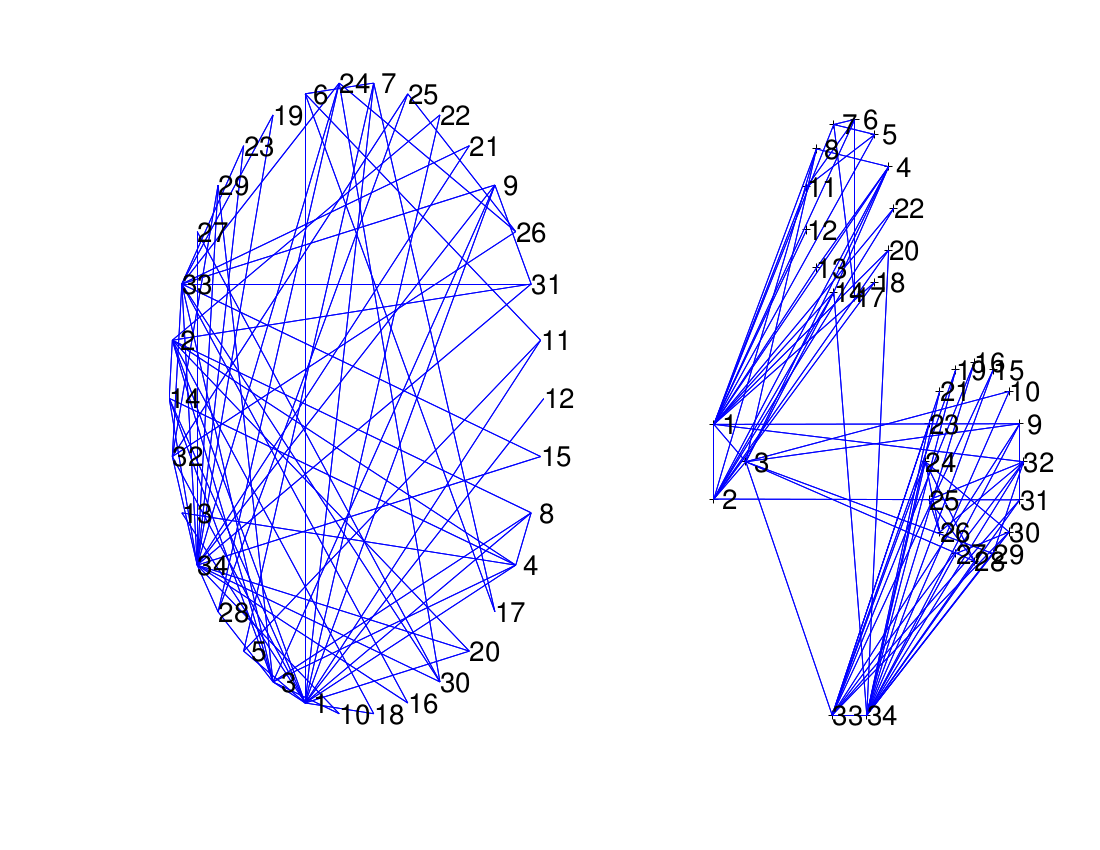
\epsfig{file = /RECHERCHE/RESEAUX/EXPOSES/FIGURES/Karate-Graph.eps,
        width=10cm, height=20cm, clip=, angle=270}
    \end{tabular}
    }
\end{tabular}
$$

%%%%%%%%%%%%%%%%%%%%%%%%%%%%%%%%%%%%%%%%%%%%%%%%%%%%%%%%%%%%%%%%%%%%%%
\newpage
$$
\vspace{-2cm}
\begin{array}{cc}
  \begin{tabular}{p{12cm}}
    \paragraph{Mixture model for random graph.} \\
    \\
    Assume the vertices (proteins, reactions) are spread into $Q$
    classes, with proportions $\alpha_q$. \\
    \\
    Assume that the probability for two vertices to be connected
    depends on the class they belong to:
    $$
    \Pr\{\i \leftrightarrow j \;|\; i \in q, j \in \ell\} = \pi_{ql}
    $$
    \\
    \paragraph{Reaction graph of {\sl E. coli}.}
    Groups 1 and 16 both involve pyruvate, but only group 1 involves also
    CO2 (group 7) and acetylCoA (group 10).
  \end{tabular}
  &
  \begin{tabular}{c}
    \paragraph{Adjacency matrix}\\
    \paragraph{of the reaction graph of of {\sl
        E. coli}.} \\
    \\
    \epsfig{file =
    /RECHERCHE/RESEAUX/EXPOSES/FIGURES/Ecoli-Complet-ERMG-Ward-Q21_class.eps, 
      height=12cm, width=12cm, clip=,bbllx=90, bblly=485, bburx=277,
      bbury=605.5}   
  \end{tabular}
\end{array}
$$

%%%%%%%%%%%%%%%%%%%%%%%%%%%%%%%%%%%%%%%%%%%%%%%%%%%%%%%%%%%%%%%%%%%%%%
\newpage
\noindent
\begin{tabular}{cc}
  \begin{tabular}{p{15cm}}
    \subsection{Detection of exceptional network motifs} \\
    \\
    \paragraph{\sl Shen-Orr \& al, Nat. Genet., 02:} \\
    Search for \textblue{over-represented motifs} in {\sl E. coli}
    transcriptional network. \\
    \\
    \paragraph{Strategy.} 
    \begin{enumerate}
    \item Count the number of occurrences $N$; 
    \item Resample a \textblue{large number of random networks}
      similar to {\sl E.coli}'s one (e.g. same degree for each gene);
    \item Estimate $\Esp N$ and $\Var N$;
    \item Calculate a $Z$-score: $Z = (N - \Esp N)/ \sqrt{\Var N}$;
    \item \textblue{Derive a $p$-value} implicitly based on a Gaussian
      approximation. 
    \end{enumerate}
    \\
    \paragraph{What would you do? ...}
  \end{tabular}
  &
  \begin{tabular}{c}
    \epsfig{file =
    /RECHERCHE/RESEAUX/EXPOSES/FIGURES/RegulationMotifs.ps, bbllx=82,
    bblly=89, bburx=289, bbury=600, clip=} 
  \end{tabular}
\end{tabular}


%%%%%%%%%%%%%%%%%%%%%%%%%%%%%%%%%%%%%%%%%%%%%%%%%%%%%%%%%%%%%%%%%%%%%%
%%%%%%%%%%%%%%%%%%%%%%%%%%%%%%%%%%%%%%%%%%%%%%%%%%%%%%%%%%%%%%%%%%%%%%
%%%%%%%%%%%%%%%%%%%%%%%%%%%%%%%%%%%%%%%%%%%%%%%%%%%%%%%%%%%%%%%%%%%%%%
%%%%%%%%%%%%%%%%%%%%%%%%%%%%%%%%%%%%%%%%%%%%%%%%%%%%%%%%%%%%%%%%%%%%%%
\end{document}
%%%%%%%%%%%%%%%%%%%%%%%%%%%%%%%%%%%%%%%%%%%%%%%%%%%%%%%%%%%%%%%%%%%%%%
%%%%%%%%%%%%%%%%%%%%%%%%%%%%%%%%%%%%%%%%%%%%%%%%%%%%%%%%%%%%%%%%%%%%%%
%%%%%%%%%%%%%%%%%%%%%%%%%%%%%%%%%%%%%%%%%%%%%%%%%%%%%%%%%%%%%%%%%%%%%%
%%%%%%%%%%%%%%%%%%%%%%%%%%%%%%%%%%%%%%%%%%%%%%%%%%%%%%%%%%%%%%%%%%%%%%

